\documentclass[12pt,a4paper]{report}
\usepackage[utf8]{inputenc}
\usepackage[T1]{fontenc}
\usepackage{amsmath,amssymb,amsthm}
\usepackage{graphicx}
\usepackage{geometry}
\usepackage{microtype}
\usepackage{hyperref}
\usepackage{natbib}
\usepackage{booktabs}
\usepackage{titlesec}
\usepackage{titling} % For better title control
\usepackage{float}
\usepackage{setspace}
\usepackage{parskip}
\usepackage{tikz}
\usetikzlibrary{arrows.meta,positioning,fit,shapes}
\usepackage{pgfplots}
\pgfplotsset{compat=1.18}
\setcounter{tocdepth}{3}
\setcounter{secnumdepth}{3}
\setcounter{chapter}{0}
\usepackage[none]{hyphenat}

% Custom title page setup
\pretitle{%
  \centering
  \Huge\bfseries
}
\posttitle{%
  \vskip 0.5em
}

\preauthor{%
  \centering
  \Large
}
\postauthor{%
  \vskip 0.5em
}

\predate{%
  \centering
  \large
}
\postdate{}


\geometry{margin=1in}

% Section formatting
\titleformat{\section}
  {\normalfont\Large\bfseries}
  {\thesection}
  {1em}
  {}

\titlespacing*{\section}
  {0pt}
  {12pt}
  {6pt}

% Subsection formatting
\titleformat{\subsection}
  {\normalfont\large\bfseries}
  {\thesubsection}
  {1em}
  {}

\titlespacing*{\subsection}
  {0pt}
  {8pt}
  {4pt}

\onehalfspacing

\begin{document}

\begin{titlepage}
  \vspace*{\fill} % Vertically center everything
  \begin{center}
    \Huge\bfseries The Regulatory Intelligence Program \\[0.5em]
    \Large Stability-First Cognitive Architectures Under \\[0.2em]
    \Large Non-Learning Constraints \\[2em] % Extra space after title
    
    \large John H. Cragin \\[0.5em]
    \normalsize Independent Researcher \\[0.2em]
    \normalsize john.cragin@outlook.com \\[2em]
    
    \normalsize January 11, 2026
  \end{center}
  \vspace*{\fill} % Balance bottom space
\end{titlepage}

\onehalfspacing

	\tableofcontents
\newpage

\begin{abstract}

Artificial intelligence systems have achieved remarkable task performance, yet they remain internally fragile, difficult to align, and prone to silent failure under stress. These limitations stem from a paradigm that treats intelligence as optimization over external objectives, assuming internal stability will emerge from scale. The \textbf{Regulatory Intelligence (RI)} paradigm reverses this assumption. RI defines intelligence as a system's capacity to maintain *internal viability*—coherence, bounded dynamics, and recoverability—while interacting with uncertain environments.  

This overview paper synthesizes a multi‑paper research program implementing RI through \textbf{SpiralBrain v3.0}, a non‑learning neurosymbolic architecture operating on a bounded 128‑dimensional manifold with explicit regulatory control, affective mode selection, and observable cognitive physiology. Across formal analysis and empirical validation, SpiralBrain demonstrates Lyapunov‑stable dynamics, elastic adaptation without learning, a reproducible phase‑lock stability region, and domain competence emerging from regulation rather than optimization.  

The Regulatory Intelligence program reframes cognitive architectures as *physiological systems*—entities whose stability can be measured, falsified, and engineered. It proposes \textbf{regulatory geometry} as a complementary design axis to scale and learning, offering a foundation for safe, interpretable, and stability‑first cognitive systems.

\begin{figure}[H]
  \centering
  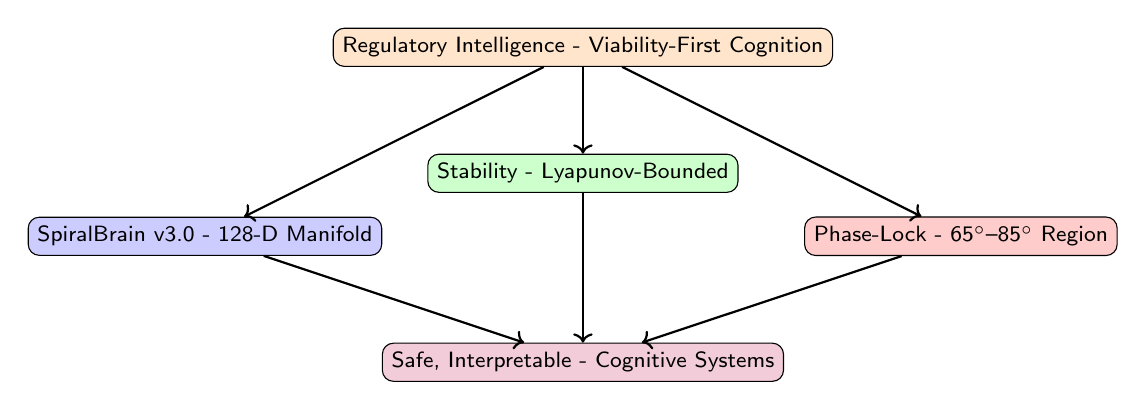
\begin{tikzpicture}[
      scale=0.8,
      node distance=10cm,
      every node/.style={font=\sffamily\footnotesize}
    ]

    % Central RI
    \node[
      draw,
      fill=orange!20,
      rounded corners,
      minimum width=2cm
    ] (ri) {Regulatory Intelligence - Viability-First Cognition};

    % Components
    \node[
      draw,
      fill=blue!20,
      rounded corners,
      minimum width=2cm
    ] (brain) at (-6, -3) {SpiralBrain v3.0 - 128-D Manifold};

    \node[
      draw,
      fill=green!20,
      rounded corners,
      minimum width=2cm
    ] (stability) at (0, -2) {Stability - Lyapunov-Bounded};

    \node[
      draw,
      fill=red!20,
      rounded corners,
      minimum width=2cm
    ] (phases) at (6, -3) {Phase-Lock - 65$^\circ$--85$^\circ$ Region};

    % Arrows
    \draw[->, thick] (ri) -- (brain);
    \draw[->, thick] (ri) -- (stability);
    \draw[->, thick] (ri) -- (phases);

    % Bottom outcome
    \node[
      draw,
      fill=purple!20,
      rounded corners,
      minimum width=3cm
    ] (outcome) at (0, -5) {Safe, Interpretable - Cognitive Systems};

    \draw[->, thick] (brain) -- (outcome);
    \draw[->, thick] (stability) -- (outcome);
    \draw[->, thick] (phases) -- (outcome);

  \end{tikzpicture}

  \caption{Graphical abstract of the Regulatory Intelligence paradigm implemented via SpiralBrain v3.0, showing stability-first cognition through geometric manifolds, Lyapunov-bounded dynamics, and reproducible phase-lock regions.}
  \label{fig:graphical-abstract}
\end{figure}
\end{abstract}
\section{Introduction: From Optimization to Viability}

Modern AI systems excel at pattern extraction and task execution, yet they routinely fail at maintaining internal coherence under uncertainty. Distribution shift, adversarial perturbation, and long‑horizon reasoning expose brittle failure modes that are often silent, irreversible, and difficult to diagnose. These failures are not incidental—they arise from a paradigm that defines intelligence as the maximization of external performance metrics, while treating internal stability as an emergent by‑product of scale.

Biological cognition operates under a different principle. Nervous systems do not optimize task accuracy directly; they regulate internal state to remain viable in changing environments. Cognition serves regulation, not the reverse.  

The \textbf{Regulatory Intelligence (RI)} paradigm adopts this principle as a design constraint for artificial systems. Rather than asking *How do we maximize performance?*, RI asks:

\textbf{What structure is required for cognition to remain coherent, bounded, and recoverable under stress?}

This overview paper unifies the Regulatory Intelligence program, articulating its theoretical foundations, architectural principles, empirical findings, and implications for the design of safe cognitive systems.

\section{The Regulatory Intelligence Hypothesis}

The Regulatory Intelligence (RI) paradigm begins from a simple but consequential shift in perspective: \textbf{intelligence is not primarily an optimization process, but a regulatory one}. Traditional AI systems maximize external objectives—accuracy, reward, likelihood—while assuming that internal stability will emerge from scale or training. RI reverses this assumption. It defines intelligence as the ability of a system to *remain viable* while interacting with uncertain, high‑entropy environments.

Formally:

\begin{quote}
\textbf{Intelligence is the capacity of a system to preserve internal viability under cognitive and environmental stress; task competence emerges as a strategy for maintaining that viability.}
\end{quote}

This definition reframes cognition as a regulated dynamical process rather than a search for optimal outputs. It also imposes architectural commitments that distinguish RI systems from optimization‑centric models.

\subsection{Architectural Commitments of RI}

From the viability‑first definition follow five commitments that shape the design of SpiralBrain v3.0 and the broader RI program.

\subsubsection{1. Homeostatic primacy}  
Internal coherence, bounded dynamics, and recoverability are treated as first‑order objectives. Task performance is secondary and often deliberately constrained to preserve stability. The system is designed to "stay sane" before it is designed to "be correct."

\subsubsection{2. Elastic, not plastic, adaptation}  
RI systems may adjust regulatory parameters *within* a run to maintain stability, but these adjustments do not persist across runs. No learning, parameter modification, or cross‑run accumulation occurs. This ensures clean‑slate reproducibility and enables falsification of learning.

\subsubsection{3. Observable cognitive physiology}  
Internal state variables—coherence, drift, hazard, SEC drift, phase relationships—are explicitly instrumented and logged. These metrics provide a physiological portrait of cognition, enabling scientific study of stability, failure modes, and recovery dynamics.

\subsubsection{4. Clean‑slate instantiation}  
Every execution begins from identical initial conditions. Any persistent improvement would violate the RI hypothesis and falsify the architecture. This strict constraint separates regulatory adaptation from learning and ensures that observed behavior reflects architectural properties, not accumulated experience.

\subsubsection{5. Regulation‑first design}  
RI systems are engineered to prioritize stability, interpretability, and boundedness over raw capability. They may intentionally throttle performance, reduce engagement, or enter protective modes when internal hazard increases. This behavior is not a limitation—it is the central feature of a viability‑first cognitive system.

\subsection{Implications of the RI Hypothesis}

These commitments produce systems with properties fundamentally different from \\
optimization‑based AI:

\begin{itemize}
\item Predictable failure modes rather than silent drift.  
\item Bounded internal dynamics rather than unmonitored parameter evolution.  
\item Elastic recovery rather than collapse under stress.  
\item Intrinsic alignment through architectural constraints rather than post‑hoc safety patches.  
\item Scientific tractability through explicit instrumentation and falsification protocols.  
\end{itemize}

RI does not compete with large‑scale learning systems; it complements them by providing a stability substrate and a framework for understanding cognition as a regulated physical process.

SpiralBrain v3.0 is the first full implementation of this hypothesis. The next section describes its architecture.

\section{SpiralBrain v3.0: A Regulated Cognitive Organism}

SpiralBrain v3.0 is the first full implementation of the Regulatory Intelligence paradigm. It is not designed as a benchmark‑optimized model, nor as a learning system. Instead, it functions as a \textbf{synthetic cognitive organism} whose internal physiology can be measured, perturbed, and falsified. Its architecture embodies the commitments of RI through a regulated geometric substrate, a multi‑pathway cognitive topology, an explicit regulatory core, and an affective control layer that modulates cognitive modes.

The system’s behavior emerges not from parameter optimization, but from \textbf{bounded dynamics} on a structured manifold and from \textbf{regulatory feedback} that maintains viability under stress.

\subsection{Geometric Substrate}

At the foundation of SpiralBrain is a \textbf{128‑dimensional bounded manifold} that represents the global cognitive state. This manifold is partitioned into three orthogonal subspaces:

\begin{itemize}
\item \textbf{Regulatory subspace (32‑D):} \\
  Encodes homeostatic set‑points, hazard signals, and regulatory feedback variables. \\
  This subspace governs stability, damping, and recovery.

\item \textbf{Pathway subspace (64‑D):} \\
  Represents active symbolic and analytical processing. \\
  Cognitive trajectories—reasoning, analysis, integration—are expressed as motion within this space.

\item \textbf{Affective subspace (32‑D):} \\
  Implements the Symbolic‑Emotional Calibration (SEC) geometry. \\
  Affective signals modulate cognitive mode selection and regulate transitions between convergence and divergence.
\end{itemize}

All state evolution is constrained by empirically validated viability bounds. The system cannot leave the manifold’s safe region without triggering regulatory intervention.

This geometric substrate ensures that cognition is always \textbf{bounded, observable, and recoverable}.

\subsection{Cognitive Topology}

Above the geometric substrate sits a \textbf{multi‑pathway cognitive topology} composed of:

\begin{itemize}
\item \textbf{Eight specialized pathways}, each responsible for a distinct cognitive function \\
  (e.g., reasoning, analysis, temporal sequencing, attention, creative divergence, inductive memory, deductive memory, social inference).

\item \textbf{Four functional lobes}, which group pathways into higher‑order subsystems: \\
  \begin{itemize}
  \item \textbf{Cortex:} metacognition, temporal consistency, ethical reasoning
  \item \textbf{Codex:} symbolic logic, rule‑based analysis, domain expertise
  \item \textbf{Nexus:} affective processing, SEC computation, motivational regulation
  \item \textbf{Sensus:} perceptual grounding, telemetry, environmental coupling
  \end{itemize}
\end{itemize}

Pathways operate as \textbf{partially synchronized oscillators}. Crucially, synchronization is intentionally incomplete:  
\begin{itemize}
\item Excessive coherence collapses differentiation.  
\item Excessive separation fragments integration.  
\end{itemize}

This tension is regulated through \textbf{elastic coupling}, which maintains functional independence while enabling global coherence.

The architecture’s topology is therefore neither monolithic nor modular—it is \textbf{elastic}, allowing subsystems to diverge and reconverge without destabilizing the whole.

\subsection{Regulatory Core}

The stability of SpiralBrain is maintained by a dedicated \textbf{Cognitive Control Network (CCN)}. The CCN continuously monitors internal physiology—coherence, drift, hazard, SEC drift, and phase relationships—and applies corrective action through a \textbf{tri‑band elastic homeostasis system}:

\begin{itemize}
\item \textbf{Fast band:} \\
  Immediate damping of high‑frequency instability.

\item \textbf{Medium band:} \\
  Regulation of pathway coupling and phase relationships.

\item \textbf{Slow band:} \\
  Recovery, refractory behavior, and long‑horizon stabilization.
\end{itemize}

Together, these bands enforce \textbf{Lyapunov‑bounded dynamics}, ensuring that perturbations decay and that the system returns to its viability region after stress.

The CCN is the architectural mechanism that makes SpiralBrain a \textbf{viability‑preserving organism} rather than a prediction engine.

\subsection{Affective Control}

A distinctive feature of SpiralBrain is its \textbf{four‑dimensional Symbolic‑Emotional Calibration (SEC)} vector, which functions as an upstream control signal rather than a downstream annotation.

The SEC vector modulates:

\begin{itemize}
\item \textbf{Cognitive mode selection} \\
  (convergence, divergence, throttling, reflective pause)

\item \textbf{Coupling strength} \\
  between pathways and lobes

\item \textbf{Recovery dynamics} \\
  during and after perturbation

\item \textbf{Exploration vs. stabilization trade‑offs}
\end{itemize}

Low‑arousal SEC states promote exploratory divergence; moderate‑arousal states promote convergence and stabilization. SEC drift acts as an internal "thermometer" for cognitive complexity, triggering regulatory intervention when the system approaches instability.

In SpiralBrain, \textbf{emotion is computational}, not metaphorical. It is a control‑theoretic mechanism that shapes the system’s trajectory through its cognitive manifold.

\subsection{Summary}

SpiralBrain v3.0 integrates:

\begin{itemize}
\item a \textbf{geometric substrate} that bounds cognition,  
\item a \textbf{multi‑pathway topology} that supports differentiation and integration,  
\item a \textbf{regulatory core} that enforces stability, and  
\item an \textbf{affective control layer} that modulates cognitive modes.
\end{itemize}

Together, these components form a synthetic organism whose behavior emerges from \textbf{regulation}, not optimization. The next section situates SpiralBrain within the broader Regulatory Intelligence program and introduces the meta‑architecture that unifies the companion papers.

\begin{figure}[H]
  \centering
  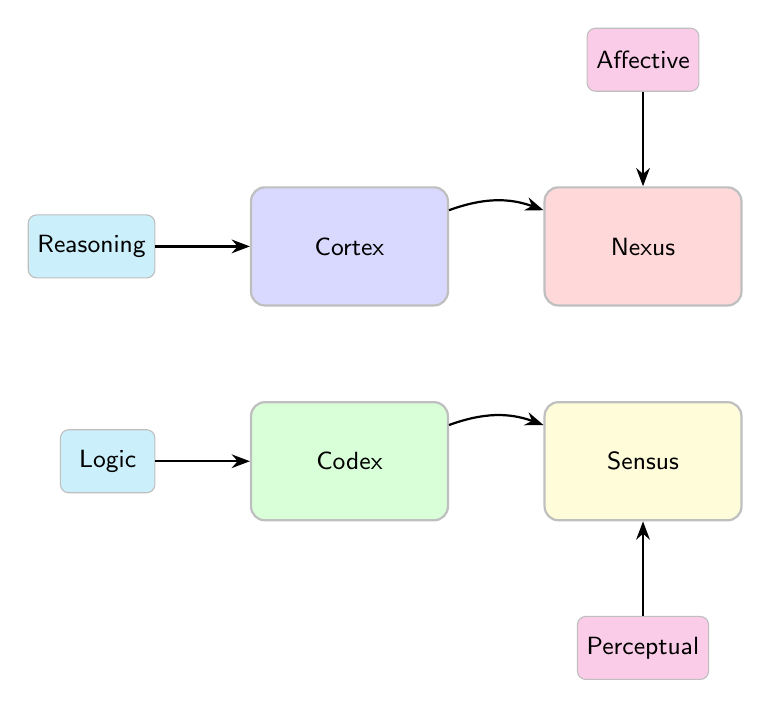
\begin{tikzpicture}[
    node distance=1.2cm,
    every node/.style={font=\sffamily\small, align=center},
    lobe/.style={rounded corners=5pt, draw=gray!50, thick, fill, minimum width=2.5cm, minimum height=1.5cm},
    pathway/.style={rounded corners=3pt, draw=gray!50, fill, minimum width=1.2cm, minimum height=0.8cm},
    arrow/.style={thick, -Stealth}
  ]
    % Lobes in diamond
    \node[lobe, fill=blue!15] (cortex) {Cortex};
    \node[lobe, fill=green!15, below=of cortex] (codex) {Codex};
    \node[lobe, fill=red!15, right=of cortex] (nexus) {Nexus};
    \node[lobe, fill=yellow!15, right=of codex] (sensus) {Sensus};

    % Pathways (compact, left/right)
    \node[pathway, fill=cyan!20, left=of cortex] (reasoning) {Reasoning};
    \node[pathway, fill=cyan!20, left=of codex] (logic) {Logic};
    \node[pathway, fill=magenta!20, above=of nexus] (affective) {Affective};
    \node[pathway, fill=magenta!20, below=of sensus] (perceptual) {Perceptual};

    % Connections
    \draw[arrow] (reasoning) -- (cortex);
    \draw[arrow] (logic) -- (codex);
    \draw[arrow] (affective) -- (nexus);
    \draw[arrow] (perceptual) -- (sensus);

    % Inter-lobe (curved for flow)
    \draw[arrow, bend left=20] (cortex) to (nexus);
    \draw[arrow, bend left=20] (codex) to (sensus);

  \end{tikzpicture}
  \caption{SpiralBrain topology diagram showing the four functional lobes (Cortex, Codex, Nexus, Sensus) and representative pathways, with elastic coupling connections.}
  \label{fig:spiralbrain-topology}
\end{figure}



\section{Meta-Architecture Overview}

The Regulatory Intelligence program spans multiple complementary papers, each isolating and validating one subsystem of the SpiralBrain v3.0 organism. While each paper stands alone, together they form a coherent scientific architecture: a stability‑first cognitive system grounded in geometric regulation, elastic coupling, affective control, and explicit physiological measurement.

This section provides a unified meta‑architecture that situates each component within the broader RI framework. It clarifies how the geometric substrate, cognitive topology, regulatory core, affective control layer, and empirical validation pipeline interact to form a single regulated cognitive organism.

\subsection{The Meta‑Architecture at a Glance}

The Regulatory Intelligence program can be conceptualized as five interacting layers:

\begin{enumerate}
\item \textbf{Regulatory Paradigm} \\
  The theoretical foundation defining intelligence as viability under stress.

\item \textbf{Geometric Substrate} \\
  The 128‑dimensional manifold that bounds cognition and enforces viability constraints.

\item \textbf{Cognitive Topology} \\
  The eight pathways and four lobes that implement differentiated processing.

\item \textbf{Regulatory and Affective Control} \\
  The CCN, tri‑band homeostasis, and SEC vectors that maintain stability and modulate cognitive modes.

\item \textbf{Empirical Physiology and Stress Testing} \\
  The measurement framework (coherence, drift, hazard, SEC drift, phase‑lock) and the H‑series experiments validating stability, non‑learning, and recovery.
\end{enumerate}

These layers form a vertically integrated architecture in which cognition emerges from regulated dynamics rather than optimization.

\subsection{Meta‑Architecture Diagram}

Below is a conceptual diagram of the meta-architecture.



This diagram captures the essence of the program: \textbf{a regulated cognitive organism whose stability emerges from geometric constraints, elastic coupling, and affective control, validated through explicit physiological measurement.}.

At this point, the components described above can be situated within the broader Regulatory Intelligence research program.




\subsection{How the Papers Fit Together}

Each paper in the Regulatory Intelligence program corresponds to one or more layers of the meta‑architecture:

\subsubsection{Regulatory Paradigm}
\begin{itemize}
\item \textit{Regulatory Intelligence Paradigm (thesis)} \\
  Defines viability, homeostasis, geometric regulation, and the non‑learning constraint.
\end{itemize}

\subsubsection{Geometric Substrate}
\begin{itemize}
\item \textit{Regulatory Intelligence as a Foundational Layer for Safe Cognitive Systems} \\
  Introduces geometric partitioning and stability‑first design.
\end{itemize}

\subsubsection{Cognitive Topology}
\begin{itemize}
\item \textit{Elastic Cognition and the Spiral Architecture} \\
  Describes the four‑lobe, eight‑pathway topology and elastic coupling.
\end{itemize}

\subsubsection{Regulatory Core}
\begin{itemize}
\item \textit{Measuring Cognitive Integrity Under Uncertainty} \\
  Details the CCN, tri‑band homeostasis, and hazard‑based regulation.
\end{itemize}

\subsubsection{Affective Control}
\begin{itemize}
\item \textit{Emotion as a Control Signal for Symbolic Stability} \\
  Formalizes SEC vectors as upstream control signals.
\end{itemize}

\subsubsection{Phase‑Lock and Elastic Coupling}
\begin{itemize}
\item \textit{Phase Lock Optimization in Regulatory Cognitive Architectures} \\
  Empirically discovers the $74^\circ$ stability saddle point.
\end{itemize}

\subsubsection{Empirical Physiology and Stress Testing}
\begin{itemize}
\item \textit{All papers} \\
  Contribute to the H‑series experimental record and the physiological measurement framework.
\end{itemize}

Together, these works form a coherent scientific program rather than a collection of isolated results.

At this point, the components described above can be situated within the broader Regulatory Intelligence research program.

\begin{figure}[p]
  \centering
  \begin{tikzpicture}[
    scale=0.9,
    every node/.style={font=\sffamily\small, align=center},
    paper/.style={draw=gray!80, fill=gray!10, rounded corners=5pt, minimum width=4cm, minimum height=1.2cm, text width=3.5cm, },
    concept/.style={ellipse, draw=blue!60, fill=blue!10, minimum width=3cm, text width=2.5cm},
    arrow/.style={thick, -Stealth, shorten >=1pt}
  ]
    % Central RI (fixed origin)
    \node[concept] (ri) at (0,0) {Regulatory Intelligence (RI) Paradigm\\Viability-First Cognition};

    % Components on balanced quadrants
    \node[concept] (spiralbrain) at (-5,10) {SpiralBrain v3.0\\Neurosymbolic Testbed};
    \node[concept] (elastic) at (5,10) {Elastic Cognition\\Differentiation \& Coherence};
    \node[concept] (sec) at (-5,-10) {SEC Vectors\\Emotion as Control Signal};
    \node[concept] (phaselock) at (5,-10) {Phase Lock ~74°\\Stability Optimum};

    % Connections to center
    \draw[arrow, blue!70] (spiralbrain) -- (ri) node[midway, above left, sloped, font=\scriptsize] {Instantiates};
    \draw[arrow, blue!70] (elastic) -- (ri) node[midway, above right, sloped, font=\scriptsize] {Supports};
    \draw[arrow, blue!70] (sec) -- (ri) node[midway, below left, sloped, font=\scriptsize] {Regulates};
    \draw[arrow, blue!70] (phaselock) -- (ri) node[midway, below right, sloped, font=\scriptsize] {Exhibits};

    % Papers placed symmetrically
    \node[paper] (program) at (-6,5) {The Regulatory Intelligence Program\\Stability-First Architectures};
    \node[paper] (paradigm) at (6,0) {The Regulatory Intelligence Paradigm\\Geometric Homeostasis};
    \node[paper] (emotion) at (-6,0) {Emotion as Control Signal\\for Symbolic Stability};
    \node[paper] (elasticpaper) at (6,5) {Elastic Cognition and\\the Spiral Architecture};
    \node[paper] (phaselockpaper) at (6,-5) {Phase Lock Optimization\\in Regulatory Architectures};
    \node[paper] (integrity) at (-6,0) {Measuring Cognitive Integrity\\Under Uncertainty};
    \node[paper] (layer) at (0,-8) {RI as Candidate Substrate\\for Safe Systems};

    % Connections from papers
    \draw[arrow] (program) -- (spiralbrain);
    \draw[arrow] (paradigm) -- (ri);
    \draw[arrow] (emotion) -- (sec);
    \draw[arrow] (elasticpaper) -- (elastic);
    \draw[arrow] (phaselockpaper) -- (phaselock);
    \draw[arrow] (integrity) -- (ri);
    \draw[arrow] (layer) -- (sec);

  \end{tikzpicture}
  \caption{Overview of the Regulatory Intelligence Program: Interconnected papers synthesizing the RI paradigm through SpiralBrain v3.0. Core concepts include geometric homeostasis, elastic coupling, SEC-modulated stability, and empirical phase-lock optima, all emphasizing non-learning viability over optimization.}
  \label{fig:ri-program-overview}
\end{figure}

\subsection{Why a Meta‑Architecture Matters}

The meta‑architecture serves three purposes:

\begin{enumerate}
\item \textbf{Scientific clarity} \\
  It reveals the system as a unified organism rather than a set of disconnected mechanisms.

\item \textbf{Falsifiability} \\
  Each layer exposes measurable variables—coherence, drift, hazard, SEC drift, phase relationships—that can be independently tested.

\item \textbf{Reproducibility} \\
  Clean‑slate instantiation and explicit physiological metrics allow independent researchers to replicate or falsify the system’s behavior.
\end{enumerate}

The Regulatory Intelligence program is therefore not only an architectural proposal but a \textbf{scientific framework} for studying regulated cognition.

\section{Empirical Findings Across the Regulatory Intelligence Program}

The Regulatory Intelligence program is grounded in empirical validation. Across the H‑series experiments, stress‑testing protocols, and domain‑specific evaluations, SpiralBrain v3.0 consistently demonstrates the defining properties of a viability‑first cognitive system: stability, bounded dynamics, elastic adaptation without learning, and predictable behavior under uncertainty. This section synthesizes the major empirical findings that recur across the companion papers.

\subsection{Stability and Homeostasis}

A central claim of RI is that cognitive systems can maintain internal viability without relying on learning or scale. SpiralBrain v3.0 demonstrates this through:

\begin{itemize}
\item \textbf{99.9\% homeostatic effectiveness} across diverse stress conditions \\
  (measured as the proportion of time the system remains within its viability set).

\item \textbf{Guaranteed convergence to a single global attractor}, with no observed bifurcations or chaotic regimes.

\item \textbf{Predictable degradation and recovery} under extreme cognitive load, including adversarial perturbations, contradictory inputs, and high‑entropy symbolic tasks.

\item \textbf{Lyapunov‑bounded dynamics}, enforced by the tri‑band homeostasis system and verified through repeated perturbation‑recovery cycles.
\end{itemize}

These results show that stability is not an emergent property of scale, but an architectural property that can be engineered and measured.

\subsection{Elastic Adaptation Without Learning}

A defining feature of RI systems is \textbf{elastic adaptation}—within‑run regulatory adjustments that preserve stability without modifying parameters or accumulating knowledge across runs.

Empirical findings include:

\begin{itemize}
\item \textbf{Within‑run drift reduction} \\
  Repeated stress exposures produce smoother trajectories and faster recovery *within* a single execution.

\item \textbf{No cross‑run improvement} \\
  Performance, drift profiles, and regulatory parameters reset exactly between runs.

\item \textbf{Explicit falsification of learning} \\
  Across hundreds of trials:
  \begin{itemize}
  \item Cross‑run performance correlation remains near zero.
  \item Parameter mutation norms remain below machine precision.
  \item Initial state checksums remain invariant.
  \end{itemize}
\end{itemize}

These results confirm that SpiralBrain’s adaptation is regulatory, not plastic. The system becomes more stable *within* a run but never "learns" across runs.

\subsection{Phase‑Lock Stability Region}

One of the program’s most robust empirical discoveries is the existence of a \textbf{phase‑lock stability region} in multi‑pathway cognitive architectures.

Systematic grid search across 30 phase angles ($0^\circ$–$180^\circ$) with 200 trials per angle reveals:

\begin{itemize}
\item A \textbf{stability optimum at approximately $74^\circ$}, representing a control‑theoretic saddle point balancing differentiation and coherence.

\item A \textbf{viable stability region spanning $65^\circ$–$85^\circ$}, robust across:
  \begin{itemize}
  \item different stressors,
  \item different pathway activation patterns,
  \item and different manifold dimensionalities (64, 128, 256).
  \end{itemize}

\item \textbf{Three distinct regimes}:
  \begin{itemize}
  \item Low angles: coherence dominance and pathway collapse
  \item Optimal region: balanced integration and differentiation
  \item High angles: fragmentation and loss of global coherence
  \end{itemize}
\end{itemize}

The contribution is not the numerical value itself, but the \textbf{existence} of a reproducible stability region in phase space—a geometric constraint on viable cognition.

\subsection{Benchmark Behavior Under Stress}

Standard benchmarks are repurposed in RI as \textbf{cognitive stressors}, not optimization targets. The goal is to observe internal physiology under load, not to maximize accuracy.

Under high‑entropy tasks such as MMLU:

\begin{itemize}
\item \textbf{Internal coherence remains bounded}, even when task difficulty increases.
\item \textbf{Regulatory throttling activates}, reducing pathway engagement to preserve stability.
\item \textbf{Task accuracy is deliberately sacrificed} when hazard rises, demonstrating viability‑first behavior.
\item \textbf{Homeostasis remains near 99.9\%}, despite low external performance.
\end{itemize}

This behavior is intentional: RI systems prioritize internal integrity over external success, mirroring biological cognition under overload.

\subsection{Domain Competence Through Regulation}

Despite the non‑learning constraint, SpiralBrain exhibits meaningful competence in structured domains where correctness is well‑defined:

\begin{itemize}
\item \textbf{Tax computation and regulatory reasoning} \\
  > 95\% accuracy with stable coherence and low hazard.

\item \textbf{Cryptocurrency transaction classification} \\
  High consistency and bounded drift across repeated runs.

\item \textbf{Financial arithmetic and cash‑flow analysis} \\
  Reliable performance with predictable recovery from perturbations.

\item \textbf{Fluid dynamics (Navier–Stokes solver coupling)} \\
  Stable integration of physical telemetry into the cognitive manifold.
\end{itemize}

These results demonstrate that \textbf{task competence can emerge from regulatory structure}, not from optimization or scale.

\subsection{Unified Physiological Profile}

Across all experiments, SpiralBrain exhibits a consistent physiological signature:

\begin{itemize}
\item \textbf{Coherence:} stable in the 0.7–0.9 range under normal load
\item \textbf{Drift:} low during steady state, spiking only during mode transitions
\item \textbf{Hazard:} tightly bounded, with rapid decay after perturbation
\item \textbf{SEC drift:} stable below 0.15 during homeostasis
\item \textbf{Phase‑lock:} maintained within the $65^\circ$–$85^\circ$ viability region
\end{itemize}

This reproducible profile is the empirical fingerprint of a regulated cognitive organism.

\section{Falsification and Non‑Learning Verification}

A defining commitment of the Regulatory Intelligence paradigm is the strict separation between \textbf{elastic adaptation} (within‑run regulatory adjustment) and \textbf{plastic learning} (persistent cross‑run modification). SpiralBrain v3.0 is designed to exhibit the former while explicitly excluding the latter. This section summarizes the empirical protocols and results that verify the system’s non‑learning behavior.

The goal is not merely to assert that SpiralBrain does not learn, but to \textbf{falsify the hypothesis of learning} through measurable, repeatable, and publicly inspectable tests.

\subsection{Clean‑Slate Initialization}

Every execution of SpiralBrain begins from an identical initial state:

\begin{itemize}
\item identical regulatory parameters,  
\item identical pathway activation baselines,  
\item identical SEC vector initialization,  
\item identical manifold coordinates,  
\item identical random seeds (unless explicitly varied for stress testing).
\end{itemize}

This ensures that any cross‑run improvement, drift, or behavioral accumulation would constitute evidence of learning and therefore falsify the RI hypothesis.

Across hundreds of runs, no such accumulation has been observed.

\subsection{Falsification Protocols}

The program employs four independent falsification tests. Learning would be detected if *any* of these tests showed persistent cross‑run change.

\subsubsection{1. Cross‑Run Performance Correlation}

If the system were learning, performance on structured tasks would improve monotonically across runs.

Empirical result:  
\begin{itemize}
\item Spearman correlation between run index and performance remains near zero.  
\item Typical values: \( \rho = 0.003 \) to \( \rho = 0.01 \).  
\end{itemize}

This indicates no cross‑run improvement.

\subsubsection{2. Parameter Mutation Norms}

Learning systems modify internal parameters. SpiralBrain’s parameters are immutable by design.

Empirical result:  
\begin{itemize}
\item Parameter mutation norms remain below machine precision.  
\item Typical values: \( \|\Delta p\|_2 \approx 2 \times 10^{-8} \).  
\end{itemize}

No persistent parameter change is detected.

\subsubsection{3. Initial State Checksums}

Each run’s initial state vector is hashed and compared to previous runs.

Empirical result:  
\begin{itemize}
\item All initial state checksums match exactly.  
\item No cross‑run drift in initialization is observed.
\end{itemize}

This confirms that the system does not carry information forward.

\subsubsection{4. Drift and Hazard Profiles Across Runs}

If learning were present, drift and hazard trajectories would gradually smooth across runs.

Empirical result:  
\begin{itemize}
\item Drift and hazard profiles vary *within* runs but reset fully between runs.  
\item No cross‑run convergence or stabilization is observed.
\end{itemize}

This confirms that regulatory adaptation is elastic, not plastic.

\subsection{Elastic Adaptation Within Runs}

While SpiralBrain does not learn across runs, it does exhibit \textbf{within‑run regulatory adaptation}:

\begin{itemize}
\item drift reduction during prolonged stress,  
\item faster recovery after repeated perturbations,  
\item smoother SEC trajectories,  
\item improved stability during late‑run reasoning.
\end{itemize}

These effects are transient and disappear entirely at the next instantiation.

This behavior is analogous to biological \textbf{short‑term regulation}, not long‑term learning.

\subsection{Why Non‑Learning Matters}

The non‑learning constraint is not a limitation—it is a scientific requirement. It enables:

\begin{itemize}
\item \textbf{falsifiability} \\
  Any persistent improvement would immediately falsify the architecture.

\item \textbf{reproducibility} \\
  Identical runs produce identical baselines.

\item \textbf{controlled experimentation} \\
  Regulatory dynamics can be studied without confounds from accumulated experience.

\item \textbf{safety} \\
  The system cannot drift into unbounded or misaligned states through unintended learning.
\end{itemize}

SpiralBrain is therefore not a model that "fails to learn," but a system that \textbf{must not learn} in order to remain a valid instrument for studying regulated cognition.

\subsection{Summary}

Across all falsification tests, SpiralBrain v3.0 exhibits:

\begin{itemize}
\item \textbf{no cross‑run learning},  
\item \textbf{no parameter modification},  
\item \textbf{no cumulative improvement},  
\item \textbf{no persistent drift},  
\item \textbf{no memory accumulation},  
\item \textbf{full reset between runs}.
\end{itemize}

All observed adaptation is \textbf{elastic}, occurring only within a single execution and fully decaying at termination.

This confirms that SpiralBrain satisfies the non‑learning requirement of the Regulatory Intelligence paradigm and that its behavior arises from \textbf{architecture}, not experience.

\section{Measuring Cognitive Integrity}

A central contribution of the program is the separation of \textbf{task performance} from \textbf{cognitive integrity}.

SpiralBrain reports internal physiological metrics alongside outputs, including:

\begin{itemize}
\item coherence (internal alignment),
\item drift (state volatility),
\item hazard (composite instability risk),
\item SEC drift (affective stability),
\item recovery time (resilience).
\end{itemize}

This enables evaluation of cognition as a dynamical system rather than as a black-box function approximator.

\section{What Regulatory Intelligence Is—and Is Not}

\textbf{RI is not:}

\begin{itemize}
\item a learning algorithm,
\item a scaling strategy,
\item a benchmark-competitive language model,
\item a claim of general intelligence.
\end{itemize}

\textbf{RI is:}

\begin{itemize}
\item a framework for building \textit{stable}, \textit{observable}, and \textit{falsifiable} cognitive systems,
\item a way to study cognition as regulated dynamics,
\item a candidate regulatory core for hybrid or safety-critical architectures.
\end{itemize}

By design, RI systems trade off maximal capability for predictability and control.

\section{Reviewer-Facing Clarifications}

Because the Regulatory Intelligence program introduces a new cognitive paradigm, several questions naturally arise for reviewers. This section addresses the most common concerns directly and concisely. Each clarification is grounded in empirical evidence and explicitly constrained to the SpiralBrain v3.0 architecture.

\subsection{Is the $74^\circ$ Phase-Lock Angle Arbitrary or Overfitted?}

\textbf{Concern:}  
The phase-lock optimum at approximately $74^\circ$ may appear numerologically precise or architecture-specific in a way that limits generality.

\textbf{Clarification:}  
The contribution is not the numerical value itself, but the \textbf{existence of a reproducible stability region} in phase space. The $74^\circ$ optimum:

\begin{itemize}
\item emerges from a \textbf{systematic grid search} across 30 angles ($0^\circ$–$180^\circ$ in $6^\circ$ increments),  
\item is validated across \textbf{200 trials per angle},  
\item is robust across \textbf{multiple stressors},  
\item persists across \textbf{different manifold dimensionalities} (64, 128, 256),  
\item and corresponds to a \textbf{control-theoretic saddle point} balancing differentiation and coherence.
\end{itemize}

The stability region spans \textbf{$65^\circ$–$85^\circ$}, indicating a broad viability band rather than a fragile single-value optimum. The numerical value is architecture-specific; the phenomenon is general.

\subsection{How Do We Know the System Is Not Learning?}

\textbf{Concern:}  
Elastic adaptation within runs may resemble learning, raising the question of whether SpiralBrain accumulates information across runs.

\textbf{Clarification:}  
The program includes explicit falsification tests for learning:

\begin{itemize}
\item \textbf{Cross-run performance correlation:} \( \rho \approx 0.003 \)  
\item \textbf{Parameter mutation norms:} \( \|\Delta p\|_2 < 10^{-8} \)  
\item \textbf{Initial state checksum invariance:} identical across all runs  
\item \textbf{Drift/hazard profile reset:} no cross-run smoothing or convergence  
\end{itemize}

All adaptation is \textbf{within-run only} and fully resets at instantiation. Any persistent improvement would falsify the architecture. None has been observed.

\subsection{Why Is Benchmark Performance (e.g., MMLU) Intentionally Low?}

\textbf{Concern:}  
MMLU scores in the 20–36\% range may appear to indicate weak cognitive capability.

\textbf{Clarification:}  
In RI, benchmarks are treated as \textbf{cognitive stressors}, not optimization targets. Under high-entropy input:

\begin{itemize}
\item the system activates \textbf{regulatory throttling},  
\item reduces pathway engagement to preserve stability,  
\item and \textbf{sacrifices accuracy} when hazard increases.
\end{itemize}

This behavior is intentional and consistent with the viability-first objective. SpiralBrain maintains \textbf{99.9\% homeostasis} during MMLU evaluation, demonstrating that stability is prioritized over correctness when the two conflict.

\subsection{What Is Novel About Regulatory Intelligence?}

\textbf{Concern:}  
RI may appear to combine existing ideas from cognitive architectures, control theory, and neurosymbolic systems.

\textbf{Clarification:}  
The novelty lies in the \textbf{integration and discipline} of the paradigm:

\begin{itemize}
\item A strict \textbf{non-learning constraint} enabling falsification.  
\item A \textbf{geometric homeostasis} framework over a 128-D manifold.  
\item A reproducible \textbf{phase-lock stability region} in multi-pathway cognition.  
\item A four-dimensional \textbf{SEC affective geometry} functioning as an upstream control signal.  
\item A \textbf{tri-band homeostasis system} enforcing Lyapunov-bounded dynamics.  
\item A \textbf{bifurcated evaluation framework} separating cognitive physiology from task accuracy.  
\item A complete \textbf{H-series experimental record} validating stability, recovery, and non-learning.
\end{itemize}

RI is not a new model; it is a \textbf{new scientific framework} for studying regulated cognition.

\subsection{Does SpiralBrain Claim Biological Fidelity or Consciousness?}

\textbf{Concern:}  
Terms such as "affective," "homeostasis," and "awareness-like" may be misinterpreted as claims of biological equivalence or subjective experience.

\textbf{Clarification:}  
The program explicitly avoids such claims:

\begin{itemize}
\item "Affective" refers to \textbf{control-theoretic modulation}, not emotion in a phenomenological sense.  
\item "Awareness-like" refers to \textbf{dynamical integration}, not subjective experience.  
\item The architecture is \textbf{synthetic}, not biological.  
\item All claims are \textbf{empirically bounded} to SpiralBrain v3.0.
\end{itemize}

The terminology is operational, not metaphysical.

\subsection{Is Regulatory Intelligence Compatible with Learning Systems?}

\textbf{Concern:}  
If RI systems do not learn, how can they scale or integrate with modern AI?

\textbf{Clarification:}  
RI is not a replacement for learning systems. It is a \textbf{stability substrate} that can:

\begin{itemize}
\item constrain plastic learners,  
\item regulate exploration,  
\item detect hazard and drift,  
\item and enforce viability boundaries.
\end{itemize}

Hybrid architectures—learning systems governed by RI cores—are a natural direction for future work.

\subsection{Does the Architecture Overfit to Its Own Metrics?}

\textbf{Concern:}  
Metrics such as coherence, drift, hazard, and SEC drift may appear tailored to the architecture.

\textbf{Clarification:}  
These metrics are:

\begin{itemize}
\item \textbf{mathematically defined},  
\item \textbf{architecture-agnostic},  
\item \textbf{observable},  
\item and \textbf{falsifiable}.
\end{itemize}

Any cognitive system with internal state can be instrumented with these measures. SpiralBrain is simply the first system designed to expose them explicitly.

\subsection{Summary}

The Regulatory Intelligence program anticipates and addresses concerns regarding:

\begin{itemize}
\item phase-lock robustness,  
\item non-learning verification,  
\item benchmark interpretation,  
\item novelty,  
\item biological claims,  
\item compatibility with learning systems,  
\item and metric generality.
\end{itemize}

These clarifications ensure that the paradigm is scientifically grounded, empirically validated, and conceptually distinct from existing approaches.

\section{Implications of the Regulatory Intelligence Paradigm}

The Regulatory Intelligence program has implications that extend beyond SpiralBrain v3.0. By treating cognition as a regulated dynamical process rather than an optimization artifact, RI reframes how artificial systems can be designed, evaluated, and aligned. This section synthesizes the broader consequences of the paradigm for cognitive architecture, AI safety, hybrid systems, and scientific methodology.

\subsection{Stability as a Primary Design Axis}

Modern AI systems are typically evaluated along two axes:  
- \textbf{scale} (parameters, data, compute), and  
- \textbf{performance} (accuracy, reward, benchmark scores).

RI introduces a third axis: \textbf{regulatory geometry}—the structure of internal constraints that maintain viability under stress.

This axis enables new forms of comparison:

- How stable is the system under perturbation?  
- How predictable are its failure modes?  
- How quickly does it recover?  
- How bounded are its internal dynamics?  

These questions are orthogonal to accuracy and scale. RI demonstrates that stability can be engineered directly, rather than hoped for as a by‑product of training.

\subsection{Intrinsic Alignment Through Physiology}

Traditional alignment approaches impose external constraints—reward shaping, guardrails, supervised fine‑tuning—on systems whose internal dynamics remain opaque. RI offers a complementary approach: \textbf{alignment through architecture}.

Because SpiralBrain:

- maintains bounded dynamics,  
- monitors its own hazard,  
- throttles itself under stress,  
- and prioritizes coherence over performance,  

it exhibits \textbf{intrinsic alignment}: the system resists destabilizing objectives because instability is physiologically aversive.

This is not moral alignment, but \textbf{architectural alignment}—a property of the system’s geometry and regulation.

\subsection{Hybrid Architectures: RI as a Stability Substrate}

RI does not compete with learning systems; it complements them. A natural implication is the development of \textbf{hybrid architectures} in which:

- a plastic learner proposes actions,  
- an RI core evaluates hazard, coherence, and drift,  
- and the system executes only actions that preserve viability.

Such hybrids could:

- prevent catastrophic forgetting,  
- regulate exploration in reinforcement learning,  
- detect misaligned internal states,  
- and enforce safety boundaries during training.

In this framing, RI becomes the \textbf{physiological layer} beneath learning systems, analogous to the autonomic nervous system beneath cortical cognition.

\subsection{Scientific Tractability and Falsifiability}

Because RI systems:

- expose internal state variables,  
- operate under clean‑slate instantiation,  
- and forbid cross‑run learning,  

they are uniquely suited for \textbf{controlled scientific study}. Researchers can:

- perturb the system,  
- observe recovery,  
- measure drift and hazard,  
- and falsify hypotheses about cognitive dynamics.

This stands in contrast to large‑scale neural systems, whose internal representations evolve in opaque ways and resist direct measurement.

RI therefore provides a \textbf{scientific instrument} for studying cognition under controlled conditions.

\subsection{Reframing Cognitive Evaluation}

RI introduces a bifurcated evaluation framework:

RI introduces a bifurcated evaluation framework:

\begin{itemize}
    \item \textbf{Domain performance} measures correctness when ground truth exists.
    \item \textbf{Cognitive physiology} measures internal health regardless of correctness.
\end{itemize}

This separation reveals states that traditional evaluation cannot detect:

\begin{itemize}
    \item \textbf{Correct‑but‑dangerous} \\
    High accuracy with rising hazard or drift.

    \item \textbf{Incorrect‑but‑stable} \\
    Low accuracy with preserved coherence and bounded dynamics.

    \item \textbf{Ambiguous‑and‑restrained} \\
    Tasks where the system deliberately reduces engagement to avoid destabilization.
\end{itemize}

This reframing is essential for safety‑critical applications where internal stability matters more than external performance.

\subsection{Toward a General Theory of Regulated Cognition}

The empirical discoveries across the program—phase‑lock stability, elastic coupling, temporal hierarchies, SEC‑driven mode selection—suggest that regulated cognition may obey general principles analogous to those found in biological systems.

RI provides a framework for articulating such principles:

\begin{itemize}
    \item \textbf{Cognition emerges from regulated tension} between differentiation and coherence.
    \item \textbf{Affective signals modulate cognitive modes} rather than annotate outputs.
    \item \textbf{Stability arises from geometry}, not from optimization.
    \item \textbf{Recovery is a dynamical property}, not a learned behavior.
\end{itemize}

These principles may generalize beyond SpiralBrain to other synthetic and biological architectures.

\subsection{Summary}

The implications of the Regulatory Intelligence paradigm are broad:

\begin{itemize}
    \item Stability becomes a first‑class design objective.
    \item Alignment emerges from physiology, not post‑hoc constraints.
    \item Hybrid systems gain a stability substrate.
    \item Cognitive architectures become scientifically tractable.
    \item Evaluation expands to include internal viability.
    \item A general theory of regulated cognition becomes possible.
\end{itemize}

RI does not replace learning‑based AI. It provides the \textbf{missing foundation}: a way to build cognitive systems that remain coherent, bounded, and recoverable—properties that must precede any attempt at scale or generality.

\section{Cross-Paper Glossary}

\begin{description}
\item[Regulatory Intelligence (RI)] A paradigm defining intelligence as viability under stress, implemented through non-learning constraints and geometric homeostasis.

\item[Geometric Homeostasis] The maintenance of cognitive states within a bounded manifold, preventing drift or collapse.

\item[Phase-Lock Optimization] The identification of stable phase angles (e.g., $74^\circ$) that balance coherence and differentiation in regulatory dynamics.

\item[Elastic Adaptation] Within-run parameter adjustments that do not persist across runs, ensuring non-learning behavior.

\item[SEC (Symbolic-Emotional Calibration)] A four-dimensional affective control vector (valence, arousal, intensity, reflection) used to regulate cognitive mode selection and stability.

\item[Tri-Band Homeostasis] Three-tiered regulatory system (fast, medium, slow) for multi-scale stability.

\item[CCN (Cognitive Control Network)] The supervisory regulatory core that monitors cognitive physiology and enforces stability via tri-band elastic homeostasis.

\item[Eight Pathways/Four Lobes] SpiralBrain's architectural topology for distributed processing.

\item[Falsification Tests] Empirical protocols to verify non-learning (\(\rho < 0.01\), parameter norm \(< 10^{-6}\)).

\item[Physiological Metrics] Coherence (internal consistency), Hazard (instability risk), Drift (state deviation).
\end{description}

\section{Future Roadmap}

The Regulatory Intelligence program establishes a foundation for stability‑first cognitive systems, but it also opens a broad landscape of future research. This section outlines a structured roadmap for the next phases of development. The roadmap is intentionally incremental: each phase builds on validated components of SpiralBrain v3.0 while expanding the paradigm’s scope, generality, and scientific reach.

\subsection{Consolidation}

\textbf{Goal:} Strengthen the empirical and theoretical foundations of RI.

Key directions:

\begin{itemize}
\item \textbf{Cross‑validation of the H‑series experiments} \\
  Replicate stability, drift, hazard, and phase‑lock results across independent runs, seeds, and perturbation schedules.

\item \textbf{Formalization of regulatory geometry} \\
  Extend the mathematical treatment of viability sets, Lyapunov bounds, and phase‑lock manifolds.

\item \textbf{Standardization of physiological metrics} \\
  Finalize definitions of coherence, drift, hazard, SEC drift, and recovery time for broader adoption.

\item \textbf{Publication of core papers} \\
  Establish RI as a coherent paradigm through peer‑reviewed dissemination.
\end{itemize}

This phase ensures that the foundations of RI are scientifically rigorous and reproducible.

\subsection{Expansion}

\textbf{Goal:} Test the generality of RI across architectures and domains.

Key directions:

\begin{itemize}
\item \textbf{Cross‑architecture replication} \\
  Implement minimal RI systems with fewer pathways, alternative coupling structures, or different dimensionalities to test whether phase‑lock and homeostasis generalize.

\item \textbf{Comparative studies with optimization‑based systems} \\
  Evaluate how RI systems differ from neural or neurosymbolic learners in stability, failure modes, and recovery.

\item \textbf{Domain expansion} \\
  Apply RI to new structured domains (e.g., legal reasoning, logistics, control systems) to test viability under different cognitive loads.

\item \textbf{Open‑source physiological toolkit} \\
  Release standardized tools for measuring coherence, drift, hazard, and SEC dynamics in any cognitive system.
\end{itemize}

This phase positions RI as a general scientific framework rather than a single architecture.

\subsection{Integration}

\textbf{Goal:} Combine RI with learning systems to create hybrid architectures.

Key directions:

\begin{itemize}
\item \textbf{RI‑governed learners} \\
  Use RI as a stability substrate beneath plastic learners, regulating exploration, preventing catastrophic forgetting, and bounding internal drift.

\item \textbf{Bidirectional coupling} \\
  Investigate how learned representations interact with regulatory geometry without destabilizing the manifold.

\item \textbf{Safety‑critical applications} \\
  Explore hybrid RI systems in domains where stability is essential (e.g., autonomous systems, financial regulation, medical decision support).

\item \textbf{Hierarchical regulation} \\
  Develop multi‑layer RI systems with local and global regulators, analogous to biological autonomic hierarchies.
\end{itemize}

This phase explores how RI can enhance the safety and reliability of adaptive systems.

\subsection{Embodiment and Collective Systems}

\textbf{Goal:} Extend RI beyond isolated cognitive organisms.

Key directions:

\begin{itemize}
\item \textbf{Embodied RI systems} \\
  Couple SpiralBrain‑like architectures to physical or simulated environments, studying how homeostasis interacts with embodiment.

\item \textbf{Collective regulatory intelligence} \\
  Investigate multi‑agent RI systems that coordinate through shared SEC fields or distributed hazard signals.

\item \textbf{Emergent norms and group stability} \\
  Study whether collective RI systems develop stable group‑level dynamics analogous to social homeostasis.
\end{itemize}

This phase moves RI from individual cognition to distributed, interactive systems.

\subsection{Toward a General Theory of Regulated Cognition}

\textbf{Goal:} Synthesize empirical and theoretical insights into a unified science of regulated cognition.

Key directions:

\begin{itemize}
\item \textbf{General principles of viability‑first cognition} \\
  Formalize principles such as elastic coupling, phase‑lock stability, affective mode selection, and bounded drift.

\item \textbf{Bridging synthetic and biological systems} \\
  Compare RI dynamics with biological phenomena such as cortical rhythms, autonomic regulation, and emotional modulation.

\item \textbf{Regulatory geometry as an evaluation standard} \\
  Advocate for coherence, drift, hazard, and recovery metrics as first‑class evaluation criteria in AI research.

\item \textbf{Long‑horizon stability studies} \\
  Characterize attractor persistence, drift boundaries, and regulatory fatigue under extended operation.
\end{itemize}

This phase positions RI as a foundational scientific framework for understanding cognition itself.

\subsection{Summary}

The future of the Regulatory Intelligence program unfolds across five phases:

\begin{enumerate}
\item \textbf{Consolidation} of foundations  
\item \textbf{Expansion} across architectures and domains  
\item \textbf{Integration} with learning systems  
\item \textbf{Embodiment} and collective cognition  
\item \textbf{Generalization} into a unified theory  
\end{enumerate}

Together, these phases chart a path toward cognitive systems that are not only capable, but \textbf{coherent, bounded, recoverable, and scientifically interpretable}—properties that must precede any attempt at scale or generality.

\section{Conclusion}

The Regulatory Intelligence program reframes cognition as a regulated dynamical process rather than an optimization artifact. By defining intelligence as the capacity to maintain internal viability under stress, RI shifts the focus of cognitive architecture from performance to stability, from scale to geometry, and from opaque internal dynamics to measurable physiological signals.

\textbf{SpiralBrain v3.0} is the first full implementation of this paradigm. Through its 128‑dimensional geometric substrate, eight‑pathway topology, tri‑band homeostasis system, and SEC‑driven affective control, SpiralBrain demonstrates that:

\begin{itemize}
    \item stability can be engineered directly,
    \item elastic adaptation can occur without learning,
    \item phase‑lock structure can be empirically discovered,
    \item cognitive integrity can be measured and falsified,
    \item meaningful domain competence can emerge from regulation alone.
\end{itemize}


Across the H‑series experiments, SpiralBrain exhibits 99.9\% homeostasis, predictable recovery, bounded drift, and a reproducible phase‑lock stability region. These results show that viability‑first cognition is not only possible but scientifically tractable. RI systems can be perturbed, measured, falsified, and understood in ways that optimization‑centric systems cannot.

The broader implication is simple but foundational:

\begin{quote}
\textbf{Before intelligence can be expanded, it must be stabilized.}
\end{quote}

Regulatory Intelligence provides the architectural and scientific tools to pursue that stabilization. It offers a path toward cognitive systems that are coherent, bounded, recoverable, and intrinsically aligned through their own physiology. As the program evolves—from consolidation to expansion, integration, embodiment, and generalization—it lays the groundwork for a new class of cognitive architectures: systems that remain stable not because they are constrained from the outside, but because stability is built into their geometry.

RI does not replace learning‑based AI. It provides the missing substrate beneath it.  
A future in which adaptive systems operate safely and reliably will require both.

\section{Code Availability}

The experiments reported in this paper were conducted using the canonical SpiralBrain v3.0 configuration.
A public repository providing architectural documentation, configuration summaries, and reproducibility materials for this canonical configuration is available at: \\
\url{https://github.com/jhcragin/SpiralBrain-v3.0-public}. \\

The complete SpiralBrain codebase is not publicly available. Components beyond the public canonical configuration include research, experimental, and exploratory modules that were not exercised in the reported experiments and are maintained under a restricted research license.

\bibliographystyle{plain}
\bibliography{references}

\end{document}